\documentclass[notes]{beamer}
\usepackage[utf8]{inputenc}
\usepackage{hyperref}
\usepackage{graphicx}

\usetheme{Luebeck}
\usecolortheme{beaver}
\beamertemplatenavigationsymbolsempty
\setbeamertemplate{footline}[frame number]
\usepackage{graphicx}

\title{SOFTENG 370 Tutorial 7}
\author{Timo van Veenendaal}
\date{29 September 2020}

\begin{document}

\maketitle

\begin{frame}{Plan}
    \begin{enumerate}
        \item What is FUSE?
        \item How does FUSE work?
        \item How does the code from Assignment 2 work?
    \end{enumerate}
\end{frame}
\begin{frame}{File systems, recap}
    \begin{itemize}
        \item On Linux, all files are identifiable by their path from the root \texttt{/}. e.g. \texttt{/tmp/test}, \texttt{/home/timo/.bashrc}, ...
        \item Different paths can represent files from different places: a USB drive, the hard disk, a location on network...
        \item Each of these 'places' will have a corresponding filesystem implementation
        \item The Linux kernel's VFS (Virtual File System) resolves a path to a specific file system
        \item File systems are typically implemented as kernel modules, but this is hard
        \item Enter FUSE: FUSE is a kernel module which allows for file systems to be implemented in user space.
    \end{itemize}
\end{frame}
\begin{frame}{What happens when I run \texttt{ls} (on a FUSE filesystem)?}
    \begin{figure}
        \centering
        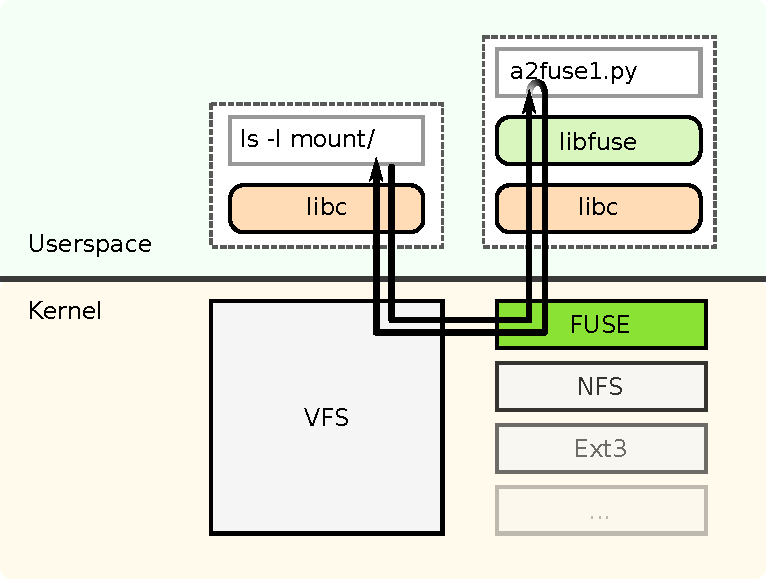
\includegraphics[width=.75\textwidth]{FUSE_structure.pdf}
        \caption{Original: CC-BY-SA 3.0, Wikipedia user Sven.}
    \end{figure}
\end{frame}
\begin{frame}{What happens when I run \texttt{ls} (on a FUSE filesystem)?}
    \begin{figure}
        \centering
        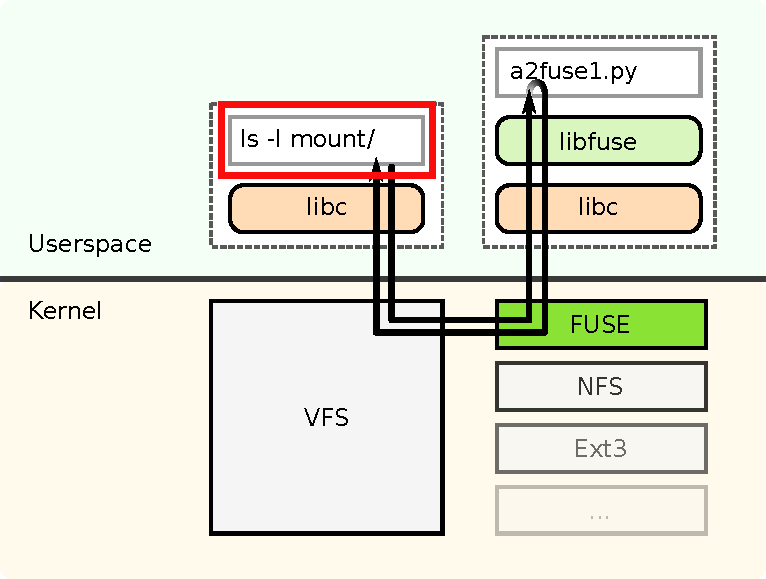
\includegraphics[width=0.6\textwidth]{FUSE_structure_ls.pdf}
    \end{figure}
    \texttt{ls} asks the C standard library (\texttt{libc}) what's in \texttt{mount/} using \texttt{readdir(3)}
\end{frame}
\begin{frame}{What happens when I run \texttt{ls} (on a FUSE filesystem)?}
    \begin{figure}
        \centering
        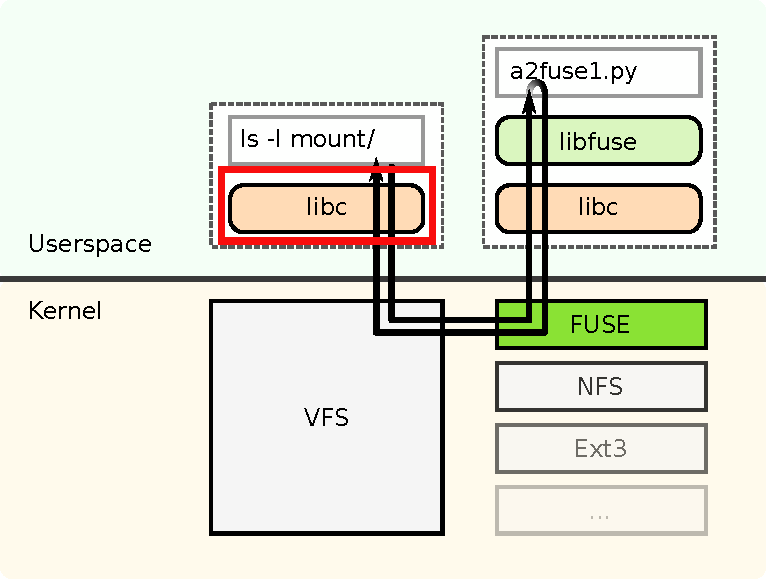
\includegraphics[width=0.6\textwidth]{FUSE_structure_libc_1.pdf}
    \end{figure}
    \texttt{libc} makes the right system calls to get this information. In particular, it uses the \texttt{readdir(2)} system call to find what files are in the directory. In doing this, it resolves the relative path provided by \texttt{ls} into an absolute path (starting with \texttt{/}).
\end{frame}
\begin{frame}{What happens when I run \texttt{ls} (on a FUSE filesystem)?}
    \begin{figure}
        \centering
        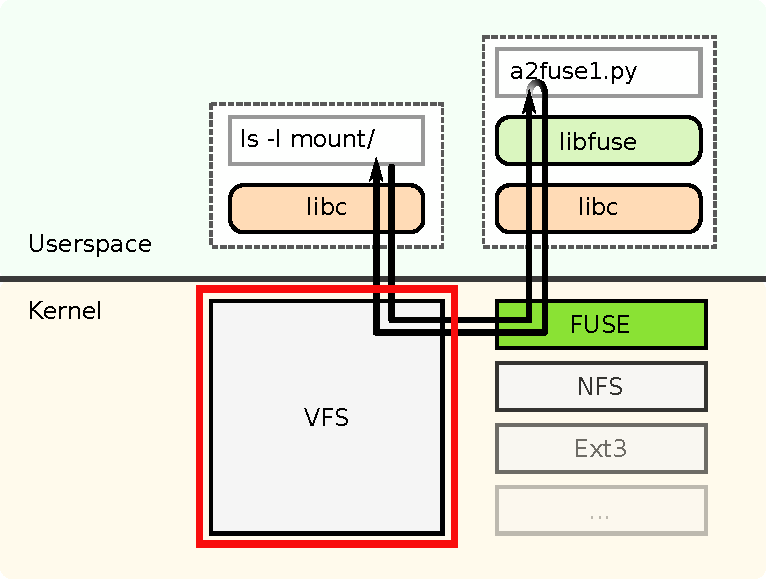
\includegraphics[width=0.6\textwidth]{FUSE_structure_vfs.pdf}
    \end{figure}
    The VFS in the kernel determines what filesystem module needs to be used to be used based on the absolute path provided. Since our FUSE filesystem is mounted at the \texttt{mount/} directory, the VFS knows it needs to go to the FUSE module. It forwards the \texttt{readdir} request to the module.
\end{frame}
\begin{frame}{What happens when I run \texttt{ls} (on a FUSE filesystem)?}
    \begin{figure}
        \centering
        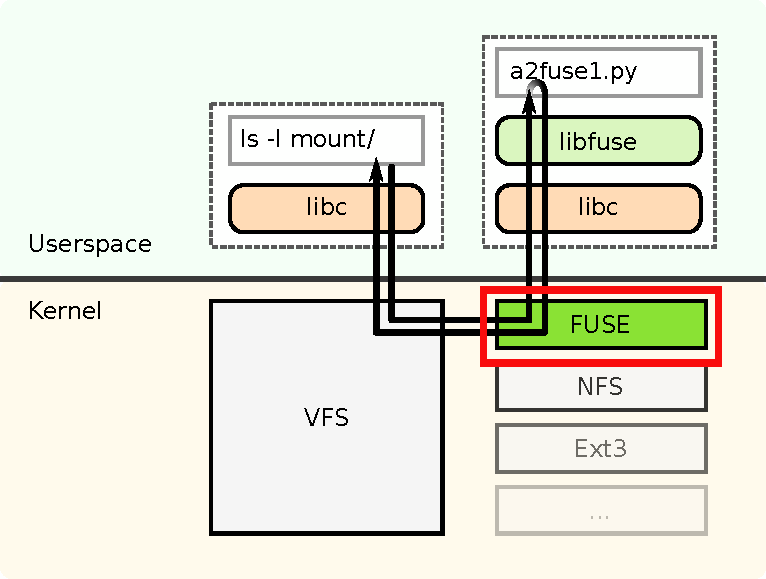
\includegraphics[width=0.6\textwidth]{FUSE_structure_fuse.pdf}
    \end{figure}
    The FUSE kernel module sends a message to the user space \texttt{libfuse} library asking for it to deal with the \texttt{readdir} request (the exact detail of how this works is unimportant).
\end{frame}
\begin{frame}{What happens when I run \texttt{ls} (on a FUSE filesystem)?}
    \begin{figure}
        \centering
        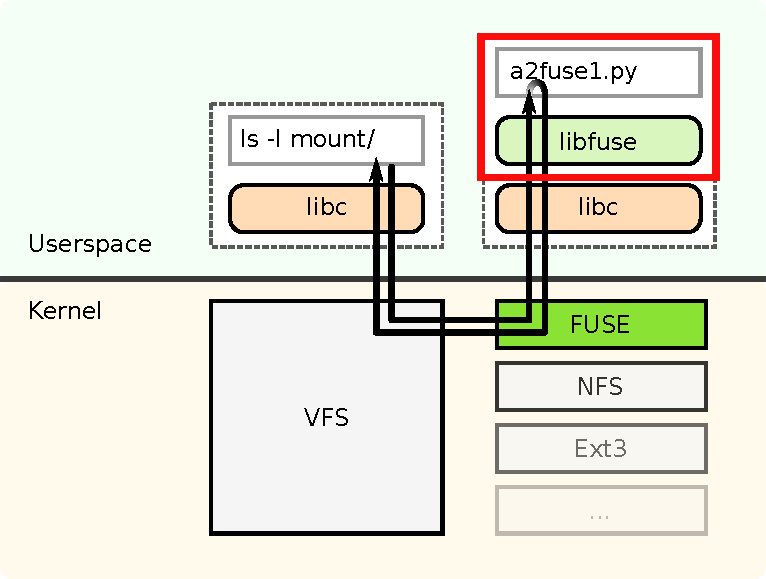
\includegraphics[width=0.6\textwidth]{FUSE_structure_libfuse.pdf}
    \end{figure}
    The \texttt{libfuse} library has a Python binding which calls the \texttt{readdir} function in your Python code. The result from the Python code is passed back through all the layers, which \texttt{ls} then uses to give its output.
\end{frame}
\begin{frame}{Generalizing this}
    \begin{itemize}
        \item This process applies for all the different filesystem operations that exist, including open, read, write, stat, and so on...
        \item You will have to implement a number of these operations for the assignment
        \item If unsure, look at how the two provided filesystems do it!
    \end{itemize}
\end{frame}
\begin{frame}{Questions?}
    Any questions?
\end{frame}
\end{document}
